\documentclass[12pt]{article}
\usepackage{amsmath,latexsym,amsfonts,amssymb,graphicx,amsthm,epsfig,enumerate}
\usepackage{tikz,verbatim,tabularx} % adds charting fuctions
\newcolumntype{C}{>{\centering\arraybackslash}X}
\linespread{1.2}

%\pagestyle{empty}

\begin{document}
	\title{6 Man's Morris: 2AA4/2ME3 Assignment 2} %add title here
	\author{
		Gregory Smilski, 1404091\\
		Abigail Gaulin, 1327924\\
		Karl Knopf 1437217} 
	% add other necessary information here
	
	\maketitle
	\thispagestyle{empty}
	\newpage
	\tableofcontents
	\newpage
	
	\section{Introduction}
	This document describes the java project 6 Men's Morris. 
	\subsection{Architecture}
	\begin{figure}[!h]
		\centering
		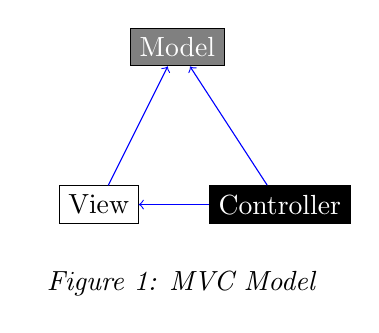
\begin{tikzpicture}
		% MVC Architecture
		\node[draw] (View) at (0,0) {View};
		\node[draw,fill=black,text=white] (Controller) at (2.3,0) {Controller};
		\node[draw,fill=gray,text=white] (Model) at (1,2) {Model};
		
		\draw[->,draw=blue] (View) to (Model);
		\draw[->,draw=blue] (Controller) to (View);
		\draw[->,draw=blue] (Controller) to (Model);
		\node at (1.0, -1.0) {\textit{ Figure 1: MVC Model}};
		
		\end{tikzpicture}
	\end{figure}
	This software uses MVC architecture in its design. MVC stands for Model, View, Controller, and is a design tool used in software development. The View contains all information the user sees, and interacts with the user. The Model contains all the data, and the Controller contains commands which modify the view and model. This architectural style is useful as it allows for modulation, and parts of the program can be modified without affecting any others.
	\subsection{Technologies}
	\begin{itemize}
		\item Java:  An object oriented programming language 
		\item Eclipse: It is an IDE used for the development and testing of software typically in Java
		\item Java Swing: A java toolkit designed to aid programmers in the creation of gui applications. This widget toolkit allows the programmer quick access to various predefined graphical objects, allowing the easy creation of a graphical interface.
		
	\end{itemize}
	\section{Modular Decomposition}
	% 4.1Description of the classes and modules and why they were used
		\begin{figure}[!h]
			\centering
			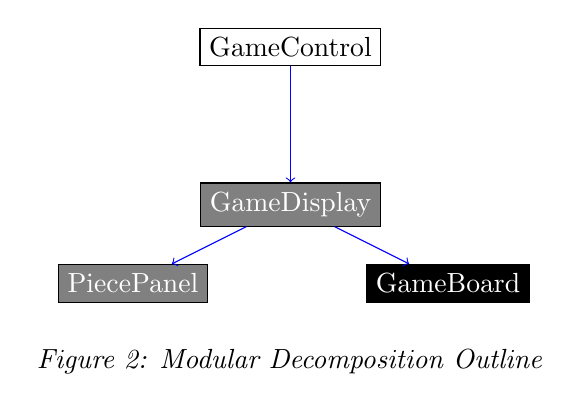
\begin{tikzpicture}
			% MVC Architecture
			\node[draw] (GameControl) at (1,3) {GameControl};
			\node[draw,fill=black,text=white] (GameBoard) at (3,0) {GameBoard};
			\node[draw,fill=gray,text=white] (GameDisplay) at (1,1) {GameDisplay};
			\node[draw,fill=gray,text=white] (PiecePanel) at (-1,0) {PiecePanel};
			
			\draw[->,draw=blue] (GameControl) to (GameDisplay);
			\draw[->,draw=blue] (GameDisplay) to (PiecePanel);
			\draw[->,draw=blue] (GameDisplay) to (GameBoard);
			\node at (1.0, -1.0) {\textit{Figure 2: Modular Decomposition Outline}};
			
			\end{tikzpicture}
		\end{figure}
	The modules chosen (as detailed in the Module Guide), were done so in order to make it straightforward for the 3 members involved in the project to code individually, and also to enforce modularity in the program. The GameDisplay, GameBoard and PiecePanel make up the View. The PiecePanel creates the tokens to take the user input, GameDisplay creates buttons to check or restart the game, and GameBoard displays the game data to the user. By dividing the View up in this way, if any of these functionalities need to be modified that can be done without affecting the other parts. The GameControl makes up the Controller. This controls the game logic, and is called by the View to make modifications to the game data based on user input. It makes sense for the Controller to be separate from the other modules, as any changes that are made to the game logic can be implemented without there being any change to what the user sees/interacts with, and likewise any changes to the user interface will not interfere with the game logic/data.
	\newpage
	\section{Module Guide}
	%4.2 For each module, a description of the interface and behaviors of each method
	\subsection{MIS}

	\begin{itemize}
		\item GameDisplay.java \\
		This module creates the Game Displayed to the window of the game. It controls the logic of the game, and calls other classes to generate the game board. \\
		\underline{Interface} \\
		\underline{Uses}
		\begin{itemize}
			\item Gameboard.java
			\item PiecePanel.java
			\item java.awt.*
			\item javax.swing.*
			\item javax.swing.border.*
			\item java.awt.event.ActionEvent
			\item java.awt.event.ActionListener
			\item java.awt.event.MouseAdapter
			\item java.awt.event.MouseEvent
			\item java.io.*
			\item java.io.PrintWriter
			\item java.util.Random
		\end{itemize} 
		\underline{Return Type}
		\begin{itemize}
			\item None
		\end{itemize}
		\underline{Access Programs}
		\begin{itemize}
			\item public GameDisplay(String title) : A constructor for the GameDisplay class. Creates an GameDisplay object with a title, that is specified by String title. This method is necessary to allow other classes to create a game display, and run the program.
			\item public GameDisplay() :Creates an GameDisplay object, using the default settings and title. Calls the public method GameDisplay(String title) to create an instance of the Game Dispaly class.
			\item public void actionPerformed(ActionEvent e): A public method that overrides the more general actionPerformed. This method specifies the actions taken when the buttons in the button panel are used.
		\end{itemize}
		\item GameBoard.java \\
		This module contains the data and specifications for displaying the 6 man's morris board to the window. It is used by Game Display to create the full game board. \\
		\underline{Interface} \\
		\underline{Uses}
		\begin{itemize}
			\item java.awt.Color;
			\item java.awt.Graphics;
			\item java.awt.Graphics2D;
			\item java.awt.Shape; 
			\item java.awt.geom.Ellipse2D;
			\item java.awt.geom.Line2D;
			\item java.awt.geom.Rectangle2D;
			\item java.util.Random;
			\item javax.swing.JPanel;
		\end{itemize} 
		\underline{Return Type}
		\begin{itemize}
			\item None
		\end{itemize}
		\underline{Access Programs}
		\begin{itemize}
			\item public Shape[][] getShapeArray() : A public method to allow other class to access the values of the shapeArray 2D array. This allows other class to see the shape of each element on the board.
			\item public void setVisibleTeams(int i, int j, int value) : A public method to allow other classes the ability to change the values of the  visibleTeams array. This allows another class to change which player controls that space (has a piece on that space).
			\item public int getVisibleTeams(int i, int j) : A public method that allows another class to get the value of the visibleTeams array at a specified i and j value. This allows another class to see which player has a piece on that space, if any.
			\item public GameBoard() : A public constructor for the class. This allows another class to be able to create a GameBoard panel for the general display.

		\end{itemize}
			\item PiecePanel.java \\
			This module contains the data and specifications for displaying the piece panel and messages to the window. It is used by Game Display to create the full game board. \\
			\underline{Interface} \\
			\underline{Uses}
			\begin{itemize}
				\item java.awt.Color;
				\item java.awt.Graphics;
				\item java.awt.Graphics2D;
				\item java.awt.Shape; 
				\item java.awt.geom.Ellipse2D;
				\item javax.swing.JPanel;
				\item javax.swing.JLabel;
			\end{itemize} 
			\underline{Return Type}
			\begin{itemize}
				\item None
			\end{itemize}
			\underline{Access Programs}
			\begin{itemize}
				\item public Shape getRedCircle() : returns the value of RedCircle.
				\item public Shape getBlueCircle() : returns the value of BlueCircle.
				\item public void setLabel(String newText) : Allows another class to set the String message to be displayed to the screen.
				\item public void setRedCount(String newText) : Allows another class to set the amount of remaining red disks to be placed.
				\item public void setBlueCount(String newText) : Allows another class to set the amount of remaining blue disks to be placed.
				\item public PiecePanel() : A constructor that allows another class to create an instance of the PiecePanel class.
				
			\end{itemize}
	\end{itemize}
		
	\subsection{MID}
	\begin{itemize}
		\item GameDisplay.java \\
		\underline{Variables}
		\begin{itemize}
			\item private static boolean isButtonNewGame : A boolean to show keep track if this is a new game.
			\item private static boolean isButtonTake : A boolean to show if a button is selected.
			\item private static boolean isButtonRecieve : A boolean to show if a button is received
			\item private boolean redTake : A boolean to show if it is Red's turn.
			\item private boolean blueTake : A boolean to show if it is Blue's turn.
			\item private PiecePanel piecePanel : A PiecePanel class to represent the pieces panel section of the display.
			\item private static GameBoard gamePanel : A GameBoard class to represent the game board section of the display.
			\item private int play1count : An integer variable representing the amount of pieces Red has left to play.
			\item private int play2count : An integer variable representing the amount of pieces Blue has left to play.
			\item private int levels : An integer representing the amount of levels in the game. For 6 Man's Morris this is 2.
			\item private int places : An integer representing the amount of places in one level of the board. For 6 Man's Morris this is 8.
			\item private int[][] current : A 2D integer array representing the amount of pieces currently on a space of the board. Should only allow one piece on each space
			\item private int currentState : An integer variable representing the current state of the game. Should only be between 0 and 4.
			\item private int previousState :An integer variable representing the previous state of the game. Should only be between 0 and 4.
			\item private int [] prevDisk : A 1D integer array representing the location of the piece that will be moved.
		\end{itemize}
		\underline{Access Programs}
		\begin{itemize}
			\item public GameDisplay(String title): A constructor for the GameDisplay, that takes a String for the title of the game.
			\item public GameDisplay() : A generic constructor for the Game Display, calls GameDisplay(String title) to construct the game display.
			\item public void actionPerformed(ActionEvent e) : A public method representing the actions taken when a button is pressed on the board.
		\end{itemize}
		\underline{Private Programs}
		\begin{itemize}
			\item private void state0() : A private method to be called when the game transitions to the first state (intial state).
			\item private void state1() :A private method to be called when the game transitions to the second state (piece placing).
			\item private void state2() :A private method to be called when the game transitions to the third state (piece moving).
			\item private void state3() :A private method to be called when the game transitions to the fourth state (milling).
			\item private void clearBoard() : A private method that is called that restarts the board, and returns to state0. 
			\item private boolean checkMill(int i,int j,int colour): A private method that checks if a mill has been achieved, returns a boolean showing if there is a mill.
			\item private void saveGame() : A private method that records the game data to a .txt file, so that it may be recovered later.
			\item private void loadGame() : A private method that load the game data from a .txt file.		
		\end{itemize}
		\item GameBoard.java \\
		\underline{Variables}
		\begin{itemize}
			\item private Shape[][] shapeArray : A 2D Shape array containing the shapes at each of the nodes on the game board. 
			\item private int[][] visibleTeams : A 2D integer array containing the values for the currrent controllers of a node on the gameboard (0-empty,1-red,2-blue).
			\item private int [][] sizingArray :A 2D integer array containing the values of the sizes of nodes on the game board. Keeps track of the scaling of each level.
			\item private double height : A private integer variable representing the height of the gameboard.
			\item private double width : A private integer variable representing the width of the game board.
		\end{itemize}
		\underline{Access Programs}
		\begin{itemize}
			\item public Shape[][] getShapeArray() : A public method allowing another class access to the values of the shapeArray variable array. Allows another class to see the shapes of each element on the game board.
			\item public void setVisibleTeams(int i, int j, int value) : A public method taking 3 integer inputs: i, the level; j, the position; and value, the value. This method the ith,jth element of the visible teams array to the value of value. Allows another class to change the elements of visibleTeams.
			\item public int getVisibleTeams(int i, int j) : A public method taking 2 integer inputs: i,the level; and j: the position. Returns the value of visibleTeams at the [i][j] position. Allows other classes to read the values of the visibleTeams array.
			\item public GameBoard() : A public constructor method that allows another class to create an instance of the GameBoard class.
			
		\end{itemize}
		\underline{Private Programs}
		\begin{itemize}
			\item protected void paintComponent(Graphics g) : An overrided method to describe how each element of game board will be coloured. 
	
		\end{itemize}
		
		\item PiecePanel.java \\
		\underline{Variables}
		\begin{itemize}
			\item private Shape redCircle : A private shape variable representing the shape of the red disk to be placed.
			\item private Shape blueCircle:A private shape variable representing the shape of the blue disk to be placed.
			\item private boolean blueTake: A private boolean variable representing if it is currently blue's turn.
			\item private boolean redTake:A private boolean variable representing if it is currently red's turn.
			\item private static boolean isButtonAdded:A private boolean representing if a button is to be added.
			\item private static boolean redAddedLast: A private boolean representing if red was added last.
			\item private static boolean blueAddedLast: A private boolean representing if blue was added last.
			\item private JLabel label1: A Jlabel that contains the message to be displayed to the screen.
			\item private JLabel label2: A Jlabel that contains the amount of red pieces remaining to be placed.
			\item private JLabel label3: A Jlabel that contains the amount of blue pieces remaining to be placed.
		\end{itemize}
		\underline{Access Programs}
		\begin{itemize}
				\item public Shape getRedCircle() : returns the value of RedCircle.
				\item public Shape getBlueCircle() : returns the value of BlueCircle.
				\item public void setLabel(String newText) : Allows another class to set the String message to be displayed to the screen.
				\item public void setRedCount(String newText) : Allows another class to set the amount of remaining red disks to be placed.
				\item public void setBlueCount(String newText) : Allows another class to set the amount of remaining blue disks to be placed.
				\item public PiecePanel() : A constructor that allows another class to create an instance of the PiecePanel class.
		\end{itemize}
		\underline{Private Programs}
		\begin{itemize}
			\item protected void paintComponent(Graphics g) : An overrided method to describe how each element of piece panel will be coloured. 
			
		\end{itemize}		
	\end{itemize}
	\section{Traceability}
	% 4.5 A Description of each class
	% Tablular Expressions
	\begin{tabularx}{\linewidth}{|C|C|C|}
		\hline \\
		Requirement & Module & Result \\
		\hline \\
		Random Player selected to go First & GameControl & random boolean generated to represent either player 1 or player 2 \\
		\hline \\
		Setting up Board Array & GameControl & int[][] generated to hold values at each position on array. Initially, the array is empty, representing no disks on board. \\
		\hline \\
		Checking if Board is Legal & GameControl & If there is more than one piece in a position, or too many pieces for a player on the board, an Error type is returned which holds value representing legality/error types present on board. \\
		\hline \\
		Displaying an array as a Six Men's Morris Board &
		GameBoard & Game is Displayed as a panel on a jFrame, allows for user interaction \\ 
		\hline \\
		Allowing the user to place a piece & GameBoard &
		User is able to select a location and place a piece \\
		
		\hline \\
	\end{tabularx}
		\begin{tabularx}{\linewidth}{|C|C|C|}
			\hline \\
			The pieces used in the game are red and blue & GameBoard & The gameboard draws the pieces and restricts their colors to red and blue \\
			\hline \\
			Requirement & Module & Result \\
			\hline \\
			Starting with an empty board displayed & GameBoard & All of the spaces are initial empty (black) on the gameboard. \\
			\hline \\
			New Game Button & GameDisplay & Allows user to select option to restart the board, will call GameControl. \\
			\hline \\
			Check Button & GameDisplay  & Allows user to check if current board is legal, will call GameControl. \\
			\hline \\
			User-Game Interaction & GameDisplay &Allows user to interact with game peices, make modifications to current board, will call GameControl. \\
			\hline \\
	\end{tabularx}
	
	\section{Uses Relation}
	% A diagram and brief description describing why how the stuff interacts
			\begin{figure}[!h]
				\centering
				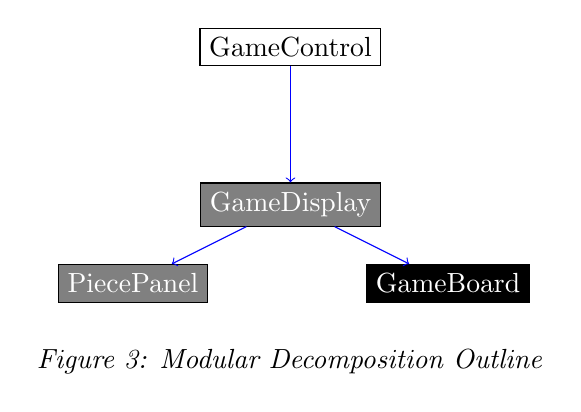
\begin{tikzpicture}
				% MVC Architecture
				\node[draw] (GameControl) at (1,3) {GameControl};
				\node[draw,fill=black,text=white] (GameBoard) at (3,0) {GameBoard};
				\node[draw,fill=gray,text=white] (GameDisplay) at (1,1) {GameDisplay};
				\node[draw,fill=gray,text=white] (PiecePanel) at (-1,0) {PiecePanel};
				
				\draw[->,draw=blue] (GameControl) to (GameDisplay);
				\draw[->,draw=blue] (GameDisplay) to (PiecePanel);
				\draw[->,draw=blue] (GameDisplay) to (GameBoard);
				\node at (1.0, -1.0) {\textit{Figure 3: Modular Decomposition Outline}};
				
				\end{tikzpicture}
			\end{figure}
	In the above relation, a class points to another that it uses.
	The View calls the Controller, which in turn modifies the Model. In the future, the View will initially take input from the user. Then, depending on which component was clicked, will call a corresponding method in the controller. Clicking either the red or blue piece will call the newpiece method in GameControl. Clicking the check button will call checkboard(), and clicking the start button will call startboard(). These methods will then modify the model through the manipulation of arrays. \\
	\newpage	
	\section{Testing}
	% A section on the testing of the software
	%Behavoir Table
	
	\begin{tabularx}{\linewidth}{|C|C|C|}
		What was Tested & What it did & Comments \\
		\hline \\
		GameControl: startboard & Printed out "current" and "teams" arrays & startboard is correctly setting up the "current" and "teams" arrays \\
		\hline \\
		GameControl: startboard & Printed out "first" boolean & "first" is correctly assigned random boolean values (on 3 separate tests was assigned true, false, and false) \\
		\hline \\
		GameControl: newpiece & Entered various input values (ie: 1,1,true) & Values were correctly entered into "current" and "teams" (ie: value of current[1][1] had 1 added to it, teams[1][1] had "a" added to it) \\
		\hline \\
		GameControl: checkboard & Ran function while no errors in array & Correctly returned no errors \\
		\hline \\
		GameControl: checkboard & Ran function while errors present & Correctly identified when too many pieces in a stack, and when a player has too many pieces on board \\
		\hline \\
		GameControl: visibleteam & Ran function with several different varieties of "teams" array (ie: when teams[0][1] = "abba") & Returned array was correct (ie: visibleteams[0][1] = "a" which is correct) \\
		\hline \\
	\end{tabularx}
	
	\begin{tabularx}{\linewidth}{|C|C|C|}
		What was Tested & What it did & Comments \\
		\hline \\
		GameBoard: GameBoard() & Display the board, allow for color change of disks & Constructor Method for the gameboard panel. Displays the board as a set of pieces. r \\
		GameBoard: GameBoard() Change Piece Color& Pieces Change color & The display was successfully able to read in the current color array. \\
	\end{tabularx}
	\begin{tabularx}{\linewidth}{|C|C|C|}
		What was Tested & What it did & Comments \\
		\hline 
		
		GameDisplay: GameDisplay() & Displayed panel in correct position in frame with buttons in correct positions in panel & GameDisplay is correctly setting up the panel \\
		GameDisplay: GameDisplay()& Clicked on "New Game?" Button,  printed "New Game!" in command line & GameDisplay is correctly running through correct output for the given input \\
		GameDisplay: GameDisplay() & Clicked on "Check!" Button, printed "Is is correct?" in command line & GameDisplay is correctly running through corect output for the given input \\
		PiecePanel: PiecePanel() & Displayed panel in correct position in frame with circle tokens in correct position in panel & PiecePanel is correctly setting up the panel \\
		PiecePanel: PiecePanel() & Clicked on Red Circle, Displayed "add red?" & PiecePanel is giving the crect output for the given input and is ready to add a red piece to the board \\
	\end{tabularx}
	\begin{tabularx}{\linewidth}{|C|C|C|}
		What was Tested & What it did & Comments \\
		\hline 
		PiecePanel: PiecePanel() &  Clicked on Blue Circle, Displayed "add blue?" & PiecePanel is giving the corect output for the given input and is ready to add a blue piece to the board \\
		PiecePanel: PiecePanel()  , Clicked on Red Circle, then white circle & White Cirtcle turned red & PiecePanel is giving the corect output for the given input and should add a red piece to the board \\
		PiecePanel: PiecePanel()  , Clicked on Red Circle, then white circle that has been coloured red & No output occurred & PiecePanel is giving the corect output for the given input and any additional red peices were not added not on their turn \\
		PiecePanel: PiecePanel()  , Clicked on Blue Circle, then white circle that has been coloured red & The red coloured white circle turned blue & PiecePanel is giving the corect output for the given input and a blue peice shoule be added \\
		PiecePanel: PiecePanel()  , Clicked on Blue Circle, then white circle & White Circle turned Blue & PiecePanel is giving the corect output for the given input and should add a blue piece to the board \\
		PiecePanel: PiecePanel()  , Clicked on Blue Circle, then white circle that has been coloured blue & No output occurred & PiecePanel is giving the corect output for the given input and any additional red peices were not added not on their turn \\
		PiecePanel: PiecePanel()  , Clicked on Red Circle, then white circle that has been coloured blue & The blue coloured white circle turned red & PiecePanel is giving the corect output for the given input and a red piece should be added \\
	\end{tabularx}
	\section{Discussion}
	%4.6 Internal review/ evaluation of design
	The design roughly follows the MVC format. The View is implented in GameDisplay, GameBoard and PiecePanel. The Controller is implemented in GameControl, which also modifies the Model. All of these parts should meet their individual requirements as shown in the Testing section.
	At present, these parts do not function together, and the connectivity of these parts will be implemented later on.
	\subsection{Anticipated Changes}
	% what was designed in anticipation of changes
	\begin{itemize}
	\item    GameControl: Will be able to track movement of pieces in the "current" and "teams" arrays (at present, can only add new pieces in). Arrays were designed to contain variables that could be modified in the future to reflect these changes.
	    In the future, the GameControl could be easily used with different dimensions (ie 8 Men's Morris).  
	\item    Error: Class designed to hold variables needed to explain what type of error is present to user of program. Returns a integer indicating the type of error, and a int[][], indicating the locations of any stack errors. Due to the design of a separate error case, if any other error types are required in the future, it will be simple to add them in.
	\item	As it currently stands, the class PiecePanel runs part of what should be in GameControl when it checks which team should be allowed to play a piece. In later versions, PiecePanel will communicate with GameControl in order to implement proper MVC design. Additionally, PiecePanel does not add actual piece objects to the board. Instead, it simply changes the colour of a test board location located between the two coloured circles. Proper adding of pieces to the board will be implemented in later versions. Also, pieces are not currently created as actual objects that can be added to the board as intended with the Piece class, so this will be changed. Finally, GameBoard does not communicate with GameControl to check if pieces are in legal locations or to start a new game. This will be implemented in later versions.
	\item Gameboard: In the near future, Gameboard() will be able to interact with the other module, using the information stored in GameControl and GameDisplay. Gameboard will also be able to succesfully check if a move is legal and be able to reset the board based on exteral commands. Some sections will be removed once they are redundant.
	\end{itemize}
	
\end{document}